\section{Proposed \textit{SocVec} Model}
\label{sec:socvec}
We first discuss the intuition behind our model informally, then present the overall workflow of our approach, and finally talk about the details of the~\textit{\socvec}~framework.

\subsection{Problem Statement and the Intuition}
We denote English as $L_1$ and Chinese as $L_2$\footnote{Thanks to the salient cross-cultural differences between the east and the west, 
we mainly consider English and Chinese. 
Nevertheless, the techniques developed here are language independent and 
thus can be used for any language pairs so long as 
necessary resources are available.}.
Given an English term $W$ and a Chinese term $U$,
the core research question is 
how to compute a \textit{cross-lingual} similarity score, $clsim(W, U)$, representing the \textit{cross-cultural} 
similarities them. 

We cannot directly calculate 
the similarity between the mono-lingual word vectors of $W$ and $U$, 
if they are trained separately and their dimensions 
are inconsistent.
We have to devise a way to compute 
similarities across two different vector spaces while retaining 
their respective social and cultural features.
That is our challenge. 

A very intuitive solution is to translate $U$ to its English 
counterpart $U'$ through a Chinese-English bilingual lexicon, and then simply compute 
the cosine similarity between $W$ and $U'$ with their English word embeddings as $clsim(W, U)$.
However, this solution is infeasible in our cases for three reasons: 
(i) if $U$ is an OOV (Out of Vocabulary) term, e.g., a slang term, 
then there is no $U'$ in the bilingual lexicon; 
%ii) if $U$ is ambiguous and has multiple translations, then the weights
%of these translated terms are hard to determine;
(ii) if $W$ and $U$ refer to the same named entity, $U' = W$, 
then $clsim(W, U)$ is just the similarity between $W$ and itself, 
therefore we cannot capture any cross-lingual differences. 
(iii) this approach does not purposely preserve the 
cultural and social context of the terms. 
%Therefore, this kind of solutions are not suitable for the two aforementioned 
%tasks, which require the cross-cultural similarities between slang terms 
and differences between entity names.

To overcome the above problems, our intuition is thus 
to project English and Chinese word vectors to a common third space, 
known as \textit{\socvec} and this projection is supposed to carry 
social and cultural context of terms.
%Considering the shortcomings of aforementioned transformation-based solutions, we propose to  
%construct a cross-lingual vector space with respect to sociolinguistic features, instead of transforming a space into another one.
%To construct a universal vector space for multilingual usage, we have to specify the meaning of each dimension for each language.
%Meanwhile, the meaning of the dimensions has to be related to opinion, sentiment, cognition and many other psychological processes to help capture the sociolinguistic information.
%Based on these two requirements, we argue that we should build a Bilingual Sociolinguistic Lexicon and extract word representation using the similarities to each translation pair in BSL as a medium.
%
\begin{figure}[t]
	\centering
	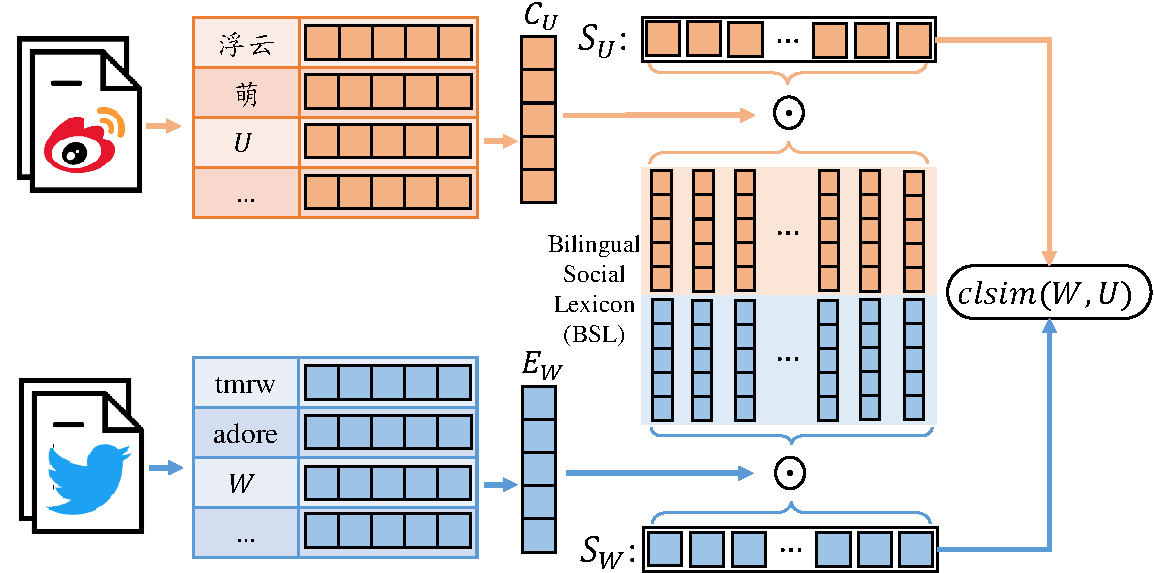
\epsfig{file=figures/framework.pdf, width=1.05\columnwidth}
	\caption{Workflow for computing the cross-cultural similarity between 
an English word \textit{W} and a Chinese word \textit{U}.}
\vspace{-15pt}
	\label{fig:overview}
\end{figure}

\begin{figure*}[th]
	\centering
	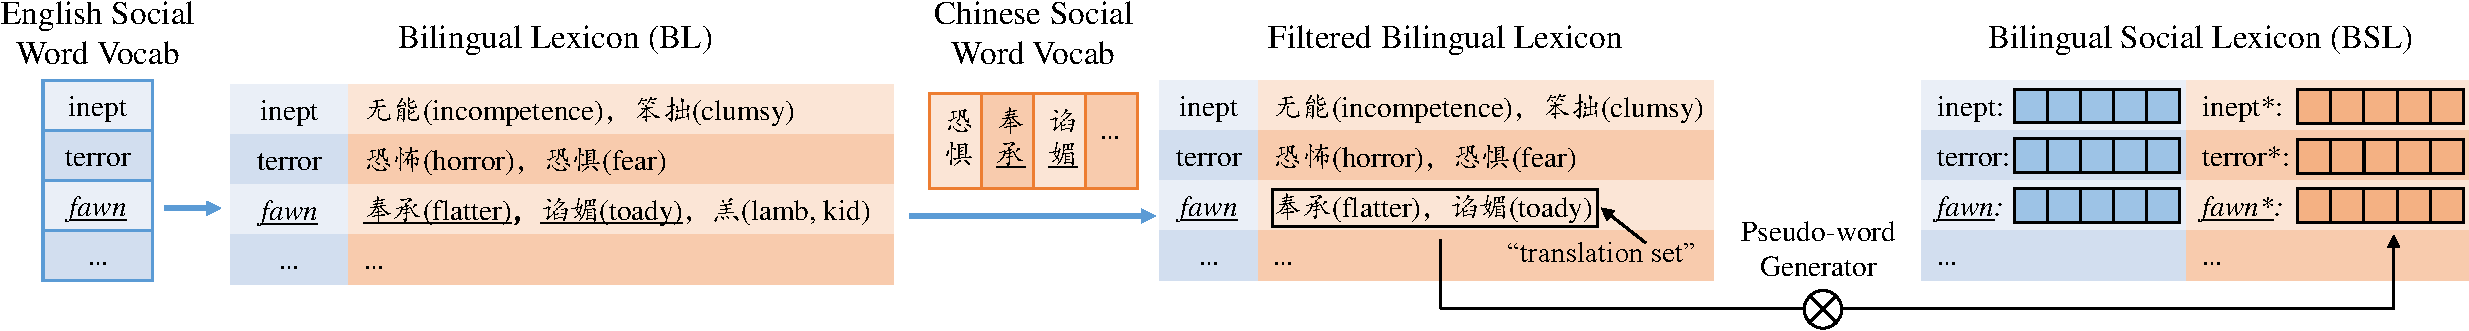
\epsfig{file=figures/BSL.pdf, width=\textwidth}
	\caption{\small Generating an entry in BSL for ``\textit{fawn}'' 
		and its pseudo-word ``\textit{fawn}*''.}
	\label{fig:BSL}
	\vspace{-10pt}
\end{figure*}
\subsection{Overall Workflow}
\figref{fig:overview} shows the workflow of our framework to construct the \textit{\socvec}~and compute $clsim(W,U)$. 
{\textbf{Notations}: \textit{CnVec} = Chinese word vector space, \textit{EnVec} = English word vector space,
	\textit{CSV} = Chinese social word vocab, \textit{ESV} = English social word vocab,
	\textit{BL} = Bilingual Lexicon, \textit{BSL} = Bilingual Social Lexicon. Finally, we denote $\bf{E_x}$, $\bf{C_x}$ and $\bf{S_x}$ as the word vectors of 
	word $x$ in \textit{EnVec}, \textit{CnVec} and \textit{\socvec} spaces
	respectively.}

The proposed \textit{\socvec}~model attacks the problem with the help of three low-cost external resources: 
i) an English corpus and a Chinese corpus from social media; ii) an English-to-Chinese bilingual lexicon (\textit{BL});  
iii) an English social word vocabulary (\textit{ESV}) and a Chinese one
(\textit{CSV}).
%For convenience, the words in these vocabularies are called
%{\em social words}. 
\footnote{Examples of social words in English include
\textit{fawn, inept, tremendous, gratitude,
terror, terrific, loving, traumatic}, etc.}
%~\footnote{There are open-sourced
%resources for these words as the following sections describe.}
%\BL{maybe use another expression for the social words} 


We train English and 
Chinese word embeddings (\textit{EnVec} and \textit{CnVec}) 
on the English and Chinese social media corpus respectively. 
Then, 
we build a \textit{BSL}
from the \textit{CSV}, \textit{ESV} and \textit{BL} (see~\secref{sec:bsl}). 
The \textit{BSL} further maps the previously incompatible \textit{EnVec} and \textit{CnVec} 
into a single common vector space \textit{\socvec~},
where two new vectors, $S_W$ for $W$ and $S_U$ for $U$,
are now comparable.
%
%\subsection{{SocVec} Modeling}
%\label{sec:model}
%In this section, we present the details of SocVec.

\subsection{Building the {BSL}}
\label{sec:bsl}
The process of building the \textit{BSL} is 
illustrated in~\figref{fig:BSL}. 
We first utilize the bilingual lexicon (BL) to translate each social word 
in the \textit{ESV} to a list of Chinese words, and then filter out all the words 
that are not in the \textit{CSV}. 
Afterwards, we have a set of 
Chinese social words for each English social word, which we denoted as a ``translation set''. Together we have a filtered bilingual lexicon now.
The final step is to generate a Chinese ``pseudo-word''\footnote{A pseudo-word can be either 
	an existing word that is the most representative word of the translation set, or a pseudo-word whose vector is computed by combining the word vectors of
	each word in the translation set.}
for each English social word using the filtered bilingual lexicon.

For example, in \figref{fig:BSL}, the
English social word ``\textit{fawn}'' has three Chinese translations in the 
bilingual lexicon, but only two of them are in CSV. 
The pseudo-word generator takes the word vectors of the two remaining words, namely
奉承 (flatter) and 谄媚 (toady), as input, and generates the pseudo-word 
vector denoted as ``\textit{fawn*}''. \footnote{Note that the direction of building \textit{BSL} can also be from Chinese to English, 
	in the same manner. However, we find that the current direction 
		gives better results due to the better quality of Enlish to Chinese translation in our BL.}
%\footnote{The reason why we use the direction from English to Chinese  is that English socio-linguistic vocabularies tend to be more accessible and accurate than low-resource languages. The filter is optional for low-resource language which has no socio-linguistic lexicon, if we can afford the inaccuracy.}

Given an English social word $s$, we denote $\mathbf{C_i}$ as 
word vector of the $i^{th}$ word of the translation set (consisting of $N$ words).
We design four intuitive types of pseudo-word generator as follows:
~\\~\\
\textbf{(1) Max.}: Maximum of the values in each dimension, assuming $K$-dimensional word vectors:
\vspace{-10pt}
{\small \begin{equation*}
	\text{Pseudo}(\mathbf{C_1},...,\mathbf{C_N}) = \begin{bmatrix}
	max(C_1^{(1)},...,C_N^{(1)}) \\
	\vdots   \\
	max(C_1^{(K)},...,C_N^{(K)})
	\end{bmatrix}^{\rm T} \\
\end{equation*}}

\noindent
\textbf{(2) Avg.}: Average of the values in each dimension:
{\footnotesize $
	\text{Pseudo}(\mathbf{C_1},...,\mathbf{C_N})=\frac{1}{N}\sum_i^N\mathbf{C_i} \
$}

\noindent
\textbf{(3) WAvg.}: Weighted average value of each dimension 
with respect to the translation confidence:
{\footnotesize $
	\text{Pseudo}(\mathbf{C_1},...,\mathbf{C_N})=\frac{1}{N}\sum_i^Nw_i \mathbf{C_i} \
$}

\noindent
\textbf{(4) Top}: Choose the most confident translation:
{\footnotesize $
	\text{Pseudo}(\mathbf{C_1},...,\mathbf{C_N}) = \mathbf{C_{top}}
$}

At the end of this step, the \textit{BSL} contains a set of English-Chinese word vector pairs, each entry representing an English social word and its Chinese pseudo-word.


\subsection{Constructing the {\socvec}~Space}
\label{sec:pg}
%\textbf{Notation Definition.} 

Let $B_i$ be an English word and $B_i^*$ be
the corresponding Chinese pseudo-word for the $i^\text{th}$ entry of \textit{BSL}.  
We can project an English word vector $\bf{E_W}$ into \textit{\socvec} by 
computing the cosine similarity between $\bf{E_W}$ and each English
word vector in \textit{BSL}, effectively constructing a new vector
$\bf{S_W}$ of size $L$. 
We also map a Chinese word vector 
$\bf{C_U}$ to be a new vector $\bf{S_U}$. 
Now $\bf{S_W}$ and $\bf{S_U}$ belong to the same vector space \textit{\socvec} 
and are comparable. 

For example, if $W$ is ``Nagoya'' and $U$ is ``名古屋'', we compute the
cosine similarities between ``Nagoya'' and each English social word in \textit{BSL}.
Such similarities compose $\bf{S_{\text{nagoya}}}$. 
Similarly, we compute the cosine similarities
between ``名古屋'' and each Chinese pseudo-words and form the social word vector $\bf{S_{\text{名古屋}}}$. 

Formally, $clsim(W,U)$ is computed as:
{\small
\begin{align*}
&clsim(W,U) := f(\mathbf{E_\text{W}},\mathbf{C_\text U}) \\ 
&=sim\left(
\begin{bmatrix}
    cos(\mathbf{E_\text W},\mathbf{E_{ B_1}})\\
    \vdots \\
    cos(\mathbf{E_\text W},\mathbf{E_{B_L}})
\end{bmatrix}^{\rm T},\begin{bmatrix}
    cos(\mathbf{C_\text U},\mathbf{C_{B_1^*}})\\
    \vdots \\
    cos(\mathbf{C_\text U},\mathbf{C_{B_L^*}})
\end{bmatrix}^{\rm T}\right)\\
&=sim(\mathbf{S_\text W},\mathbf{S_\text U}), 
\end{align*}}
\noindent where $cos$ denotes the cosine similarity.
The function $sim$ is a generic similarity function, for which a number of
metrics will be considered later in experiments.
%
%to project $\mathbf{E_W}$ and $\mathbf{C_U}$ to $\mathbf{S_W}$ and $\mathbf{S_U}$ so that they can be comparable to each other.
%We define the function $f$ to compute cross-lingual similarity between $W$ and $U$ as follows.\footnote{Here $cos$ stands for cosine similarity, } This calculation process is also shown in ~\algref{alg:alg1}. \\
%
%\begin{algorithm}[th]
%	\small
%	\DontPrintSemicolon
%	\caption{Compute cross-lingual similarity between an English word 
%		\textit{W} and a Chinese word \textit{U} } 
%	\label{alg:alg1}
%	\KwIn{ \textit{EnVec}, \textit{CnVec}, $BSL$ with $L$ word pairs} 
%	\KwOut{the cross-lingual similarity $clsim(W,U)$} 
%	$E_W$ = word vector of $W$ in \textit{EnVec}\\
%	$C_U$ = word vector of $U$ in \textit{CnVec}\\
%	$S_W$ =  zero vector with $L$ dimension \\
%	$S_U$ =  zero vector with $L$ dimension \\
%	%	\Comment*[l]{Project $E_W$ into $S_W$}
%	\For{$1 \le i \le L$}{
%		$B_i$ =  $i^{th}$ English word in \textit{BSL} \\
%		$B_i^*$ = Chinese pseudo-word of $B_i$ \\
%		$S_W[i]$ = $cos(E_W,E_{B_i})$\\
%		$S_U[i]$ = $cos(C_U,C_{B_i^*})$\\
%	} 
%	\Return $clsim(W,U)$ = $sim(S_W,S_U)$\\
%\end{algorithm}
%\begin{figure}[th!]
%	\centering
%	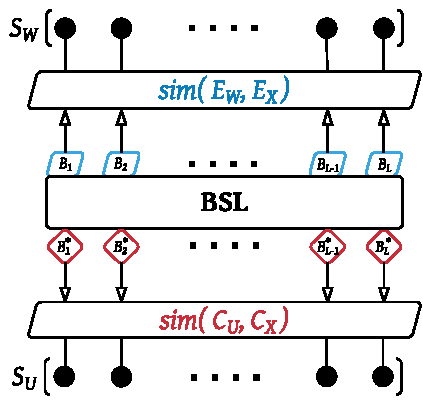
\epsfig{file=figures/SocVec.pdf, width=0.6\columnwidth}
%	\caption{Using \textit{BSL} to project $E_W$ and $C_U$ to $S_W$ and $S_U$.}
%	\label{fig:swsu}
%\end{figure}

%\subsubsection{Parameters Description}
%\label{sec:pd}
%Here, we briefly summarize the main parameters of \textit{SocVec} model:
%\begin{itemize}
%\item Two trained monolingual word embeddings, \textit{EnVec} and \textit{CnVec};  
%\item A bilingual lexicon;
%\item Chinese and English socio-linguistic vocabularies; 
%\item Pseudo-word generator function; 
%\item Option of similarity function $sim$; 
%\end{itemize} 
%We conduct several experiments for testing the these parameters in~\secref{sec:mcdne}.
